\documentclass[12pt]{article}
\usepackage{graphicx} % Required for inserting images
\usepackage[spanish]{babel}
\usepackage{lmodern}
\renewcommand{\familydefault}{\sfdefault}
\usepackage{geometry}
\usepackage{setspace}
\usepackage{float}
\usepackage{xcolor}
\usepackage{amsmath}
\usepackage{tikz}
\usepackage[colorlinks=true, urlcolor=blue]{hyperref}
\usepackage{hyperref}
\title{Practica 2 - WEB}
\author{Cerón Samperio Lizeth Montserrat}
\date{September 2025}

\begin{document}
\definecolor{azul}{RGB}{0, 168, 255}
\definecolor{azul2}{RGB}{7, 74, 163}

\begin{titlepage}
    \thispagestyle{empty}
    \newgeometry{left=2cm, right=1cm, top=2cm, bottom=2cm}
    
    % Gráfico de fondo corregido para ser fiable
    \begin{tikzpicture}[overlay, remember picture, fill opacity=0.7]
        \begin{scope}[shift={(current page.center)}]
            \rotatebox{-45}{\fill[azul2] (5, -15) rectangle (12, 15);}
            \rotatebox{-45}{\fill[azul] (3, -15) rectangle (5, 15);}
        \end{scope}
    \end{tikzpicture}
    
    \begin{spacing}{1.5}
        {\Huge \bfseries \noindent PRÁCTICA 2}
        \vspace{10pt}

        {\LARGE MÉTODOS HTTP: PUT, PATCH, DELETE, GET}
        
        \vspace{1cm}
        
        {\Large Equipo:} \\
        {\Large Beltrán Saucedo Axel Alejandro} \\
        {\Large Cerón Samperio Lizeth Montserrat} \\
        {\Large Higuera Pineda Angel Abraham} \\
        {\Large Lorenzo Silva Abad Rey} \\
        {\Large 4BV1}
    \end{spacing}
    
    \vspace{1.5cm}

    \begin{minipage}{7.5cm} % Ancho ajustado
        {\Large ESCUELA SUPERIOR DE CÓMPUTO}
    \end{minipage}

    \vfill % Empuja el contenido hacia el final de la página

    \begin{flushleft}
        {\Large \color{black}
        % Comando \textbf corregido con llaves
        \textbf{TECNOLOGÍAS PARA EL DESARROLLO DE APLICACIONES WEB}}
        
        \vspace{0.5cm}
        
        25/09/2025
    \end{flushleft}
    \vspace{1cm}
\end{titlepage}

\section{Diagrama UML}
\begin{figure}[h!]
    \centering
    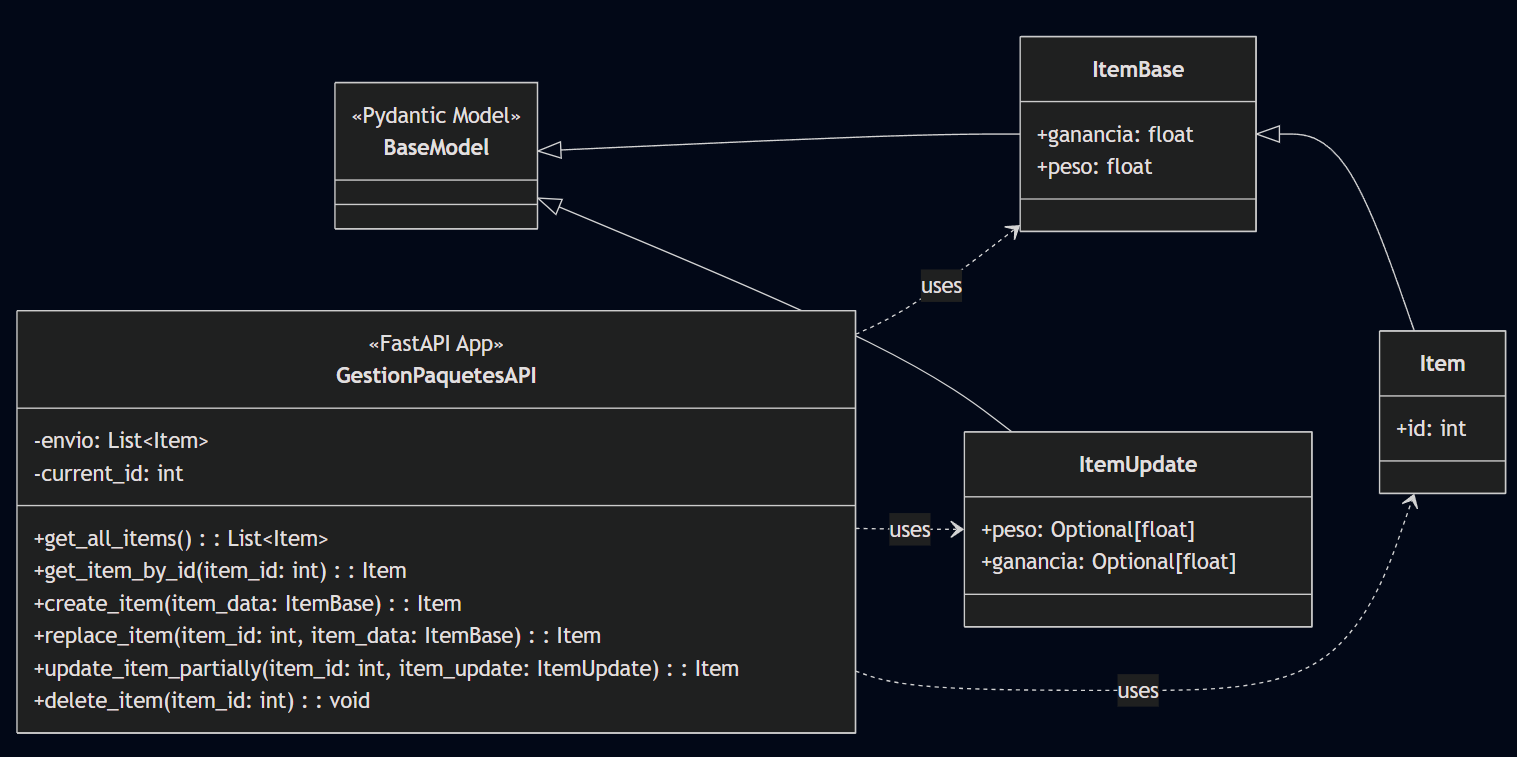
\includegraphics[width=1\textwidth]{Imagenes/Diagrama UML.png}
\end{figure}
\section{Implementación}
\begin{figure}[h!]
    \centering
    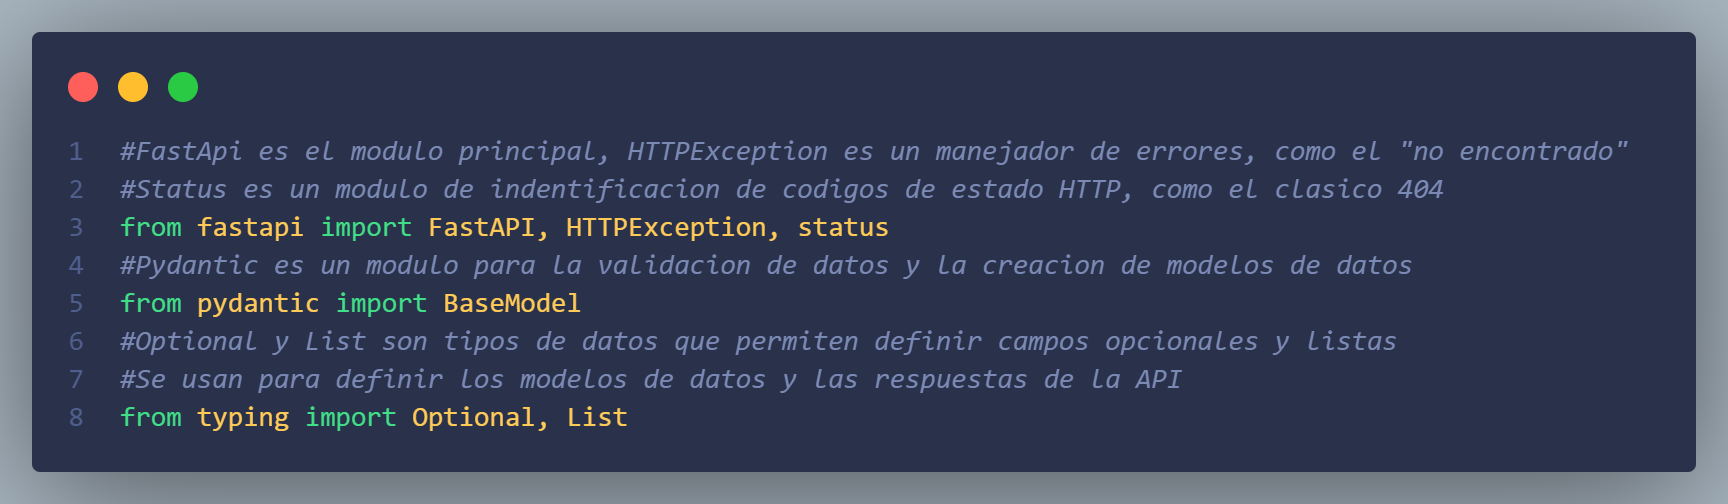
\includegraphics[width=1\textwidth]{Imagenes/Captura1_librerias.png}
\end{figure}

En este apartado se tienen los modulos a utilziar para el funcionamiento de la practica.\\
FastApi nos permite contruir APIS de manera rapida y sencilla, permitiendo definir rutas y manejar solicitudes HTTP de manera eficiente.\\
Las rutas que utilizaremos en esta practica son: GET, POST, PUT y DELETE.\\
Utilizamos Pydantic para validad entradas y para la creacion de un modelo de datos, que en es este caso sera para tener la id de un objeto, y su respectivo contenido.\\
Optional y list son tipos de datos que nos permiten definir atributos que pueden ser opcionales y listas respectivamente.\\


\begin{figure}[h!]
    \centering
    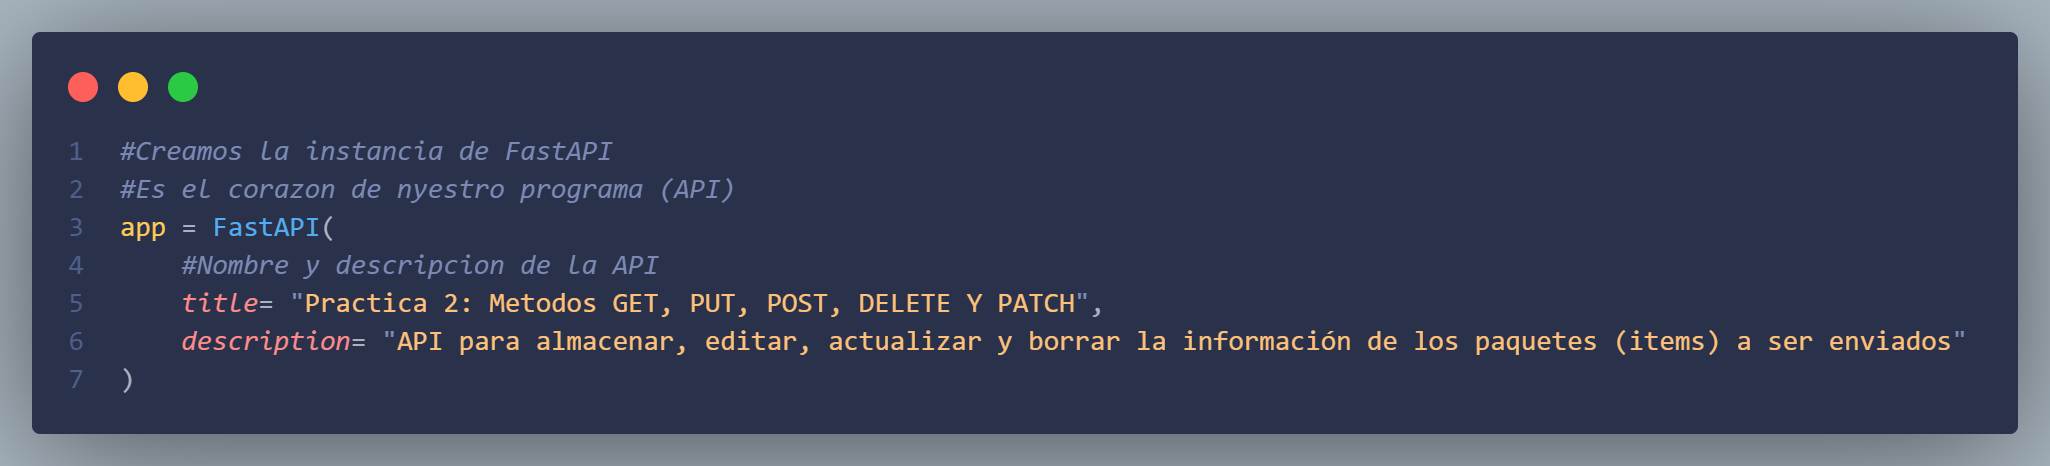
\includegraphics[width=1\textwidth]{Imagenes/Captura2_corazon del programa.png}
\end{figure}

Iniciamos con el corazon de nuestro programa, que es la instancia de FastAPI, en donde definimos el nombre y la descripcion de la API.\\

\begin{figure}[H]
    \centering
    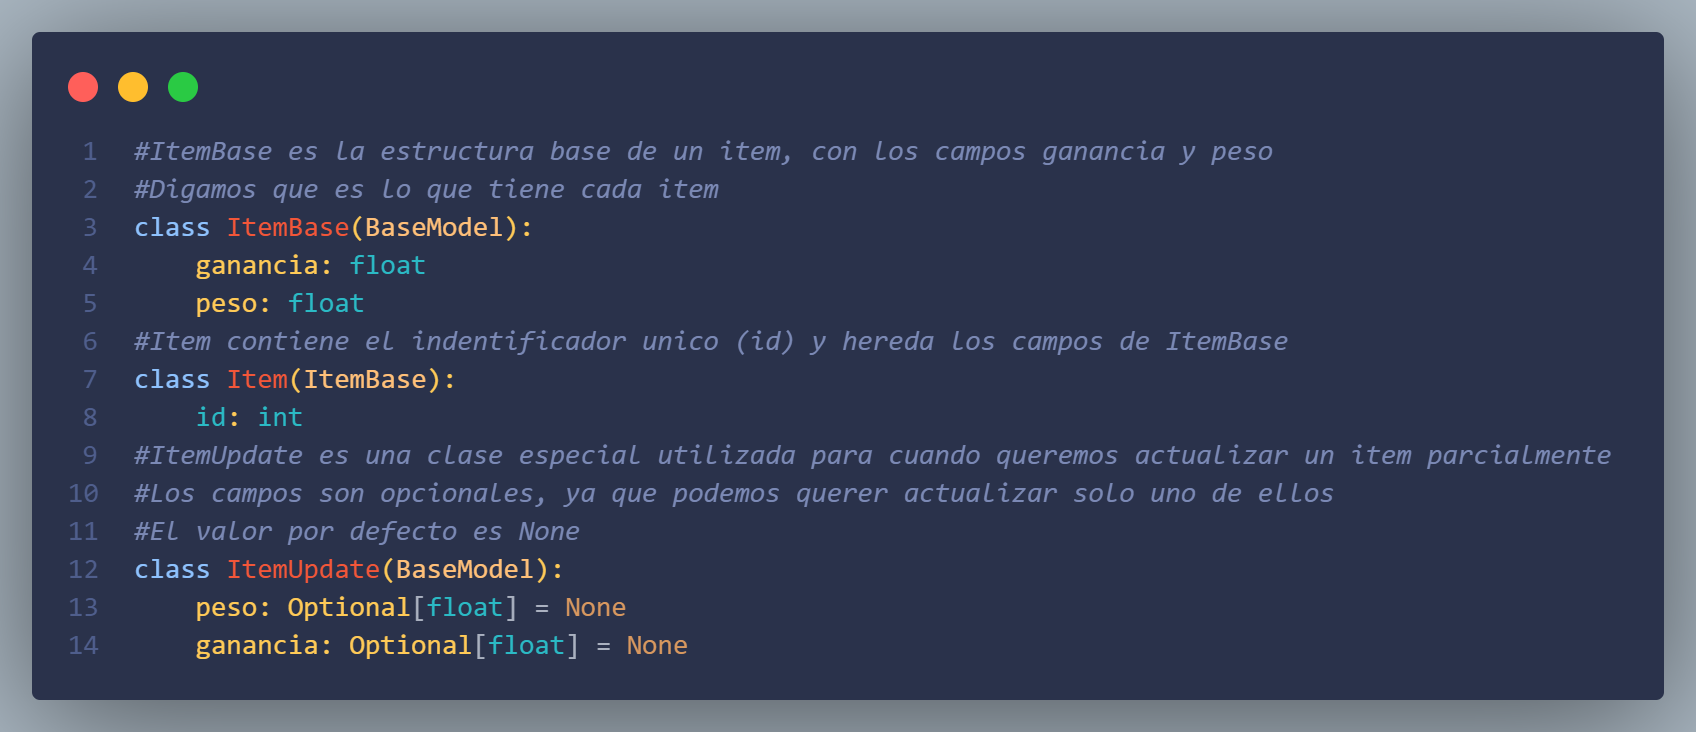
\includegraphics[width=1\textwidth]{Imagenes/Captura3_esctructuradatos.png}
\end{figure}

Gracias a Pydantic, podemos crear una estructura de datos para nuestros objetos a utilizar.
Se tiene un id de tipo entero, este servira para identificar cada objeto.
Cda objeto tiene un contenido de datos, en este caso cuenta con ganancia y perso, ambos de tipo flotante.
Además se tiene una estrcutura para actualizar los datos parcialmente, los campos son opcionales, esto es debido a que no es obligatorio actualizar ambos.

\begin{figure}[H]
    \centering
    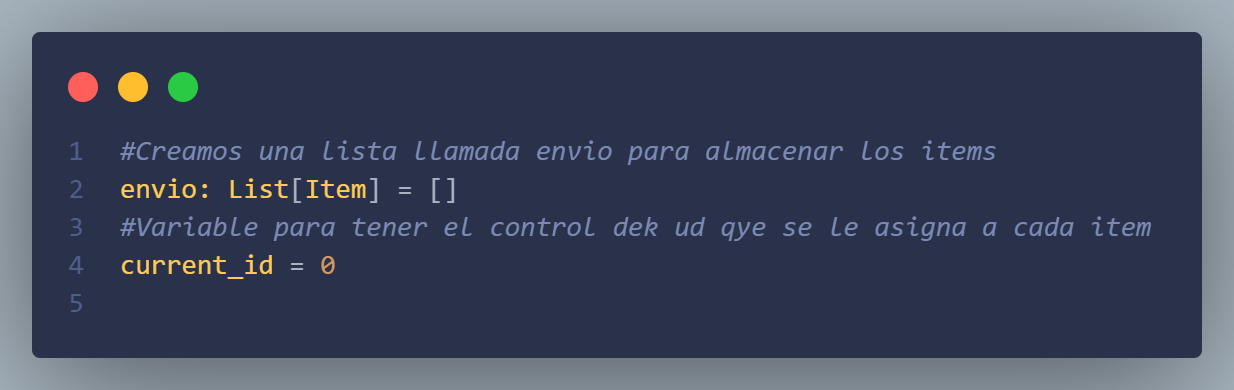
\includegraphics[width=1\textwidth]{Imagenes/Captura4_variablesGlobales.png}
\end{figure}
Utilizamos variables globales para almacenar los objetos y llevar un control del id.
El id se inicializa en 0, y se incrementa cada vez que se crea un nuevo objeto.
Los objetos se almacenan en una lista, que inicialmente esta vacia.
\end{document}